% UPDATED BY MARCUS SCHAGERBERG, 2023
% CREATED BY WOLFGANG AHRENDT, 2021

% WRITTEN BY JAKOB WINDT & MARTIN BLOM, 2023
This section will present the tools and methods used throughout the project, and how certain aspects were implemented. Firstly we explain our thought processes on choosing any existing tools, and then present any tools that were created in order to aid in the development. Lastly we present the workflow that was used, from the planning to the organisation and testing methodology.

% EDITED BY MARTIN BLOM, 2023
\section{Tools}
    In the following section we will review the software tools that significantly influenced our development process, and the motivation behind choosing these tools. Central to our discussion is the choice of Unity as our primary game engine, over other established alternatives such as Unreal Engine. We will delve into the key factors that influenced this decision, encompassing the team's familiarity with Unity's primary programming language, C\#, the advantageous size of the Unity Asset Store, and the engine's flexibility. Finally, we will provide a brief overview of how we utilised GitHub for efficient version control.

    % WRITTEN BY JAKOB WINDT, 2023
    % EDITED BY MARTIN BLOM, 2023
    \subsection{Unity}
        The traffic simulation tool is built in the Unity game engine. There are a few reasons why it was chosen as the development platform for the project, instead of a similar game engine like Unreal Engine. To begin with, C\# is the main programming language supported by Unity, which most of the team members had previous experience with. Furthermore, C\# is an inherently simpler language compared to C++, the main language of Unreal Engine, making it easier for the team members without experience to learn. Therefore, the development of the tool was started in a shorter time frame than what would have been expected had Unreal Engine been chosen as the platform.

        Another reason is Unity's larger user base, resulting in more resources such as tutorials and useful development tools. They also have a more comprehensive asset store compared to Unreal Engine, making finding models and other helpful assets likelier and easier. One of the most notable assets used is Edy's Vehicle Physics that allows for realistic vehicle physics\cite{edy}. This circumvents the need to develop a custom vehicle physics engine, instead enabling the team to use the asset to quickly configure the vehicles.

        The final reason why Unity was chosen, was due to its flexible developing structure and higher level of freedom when it comes to implementing solutions. Unity revolves around developing with scripts and conventional object oriented programming. In comparison, Unreal Engine has more advanced tools that might yield better results, although end up taking longer to learn. The level of customisation available inside the engine is greater in comparison to Unreal Engine. However, because of this, Unity ends up being more unstable whereas Unreal is far more stable and robust.

    % WRITTEN BY JAKOB WINDT, 2023
    \subsection{Third-Party Assets}
        Built into Unity is their asset store. Instead of creating everything from scratch, the team opted to utilise some assets. An asset can be anything from a 3D model to animations and scripts. Multiple assets were taken advantage of throughout the development period of the project. These assets include impactful ones such as Edy's Vehicle Physics and the Bézier Path Creator\cite{bpc}. Edy's Vehicle Physics is a package that includes a tool that allows its user to easily implement realistic vehicle physics into 3D models, while the Bézier Path Creator is a light-weight editor for creating Bézier paths in the editor. This saves a substantial amount of time since they eliminate the need to design custom tools for these tasks.

    % WRITTEN BY JAKOB WINDT, 2023
    \subsection{GitHub}
        A commonly used tool when developing software in larger groups is Git\cite{git}. Git is a free and open-source version control system that allows its users to collaborate in an easy and efficient way. 

        GitHub\cite{github} is an online software development platform that utilises Git to store and track software projects. It allows for users to work in their own separate branches, and later merge those into the main repository. This feature was used in the project. Prior to merging new code to the main repository, the code was required to be reviewed by at least one other team member to ensure that the code was well commented, functional, and that it followed the C\# coding standard.


\section{Simulation Design and Implementation}
    This section provides an overview of the development and functionality of the various software components we developed to create a traffic simulation. We delve into the use of composite Bézier curves for realistic road generation, the implementation of points of interest, and how our agents interact with these. In addition, we explain how we employed nodes for vehicles' navigation. Furthermore, we outline how we integrated the previously mentioned A* algorithm for optimised pathfinding, and how we utilised OpenStreetMap data to generate authentic cityscapes for the simulation environment.



    % WRITTEN BY HANNES KAULIO, 2023
    \subsection{Road Generation}
        Composite Bézier curves were used in order to create realistic roads with smooth curves. This can be seen in figure \ref{fig:unity-bezier-path}. A number of parameters can be changed in the Bézier path to modify the appearance. The Bézier control points will shape the road and its characteristics. The position and sharpness of a turn can be modified by changing the location of the control points.
        
        \inlineimagewithlabel{figures/method/road_generation/bezier_path_unity.png}{Composite Bézier path}{0.5}{unity-bezier-path}
    
        While the Bézier curves provides a good base for the road implementation, it is hard to build and implement logic for it since it is a continuous path. The Bézier logic and its control points were abstracted away with a node implementation in addition to the Bézier path. A number of nodes called RoadNodes are placed along the Bézier path at a rate dependent on the curvature of the road. The nodes are all connected to their previous and next nodes along the path. The goal of these nodes is to carry enough information to procedurally build the road mesh, and provide the logic needed for the agents to navigate the road network.
        \inlineimagewithlabel{figures/method/road_generation/roadnodes.png}{Visual representation of RoadNodes places along a Composite Bézier path}{0.5}{road-nodes}
    
        By using the RoadNodes, visualised in figure \ref{fig:road-nodes}, generating the road mesh is possible. The mesh is procedurally generated by placing vertices offset from the RoadNode by the width of a lane. If multiple lanes should be generated, additional vertices are added in each normal direction. Triangles are then drawn between the vertices to create the mesh. To add the road material, the lanes are split into sub meshes, making it easy to generate the road lines. The power of procedural generation is the ability to customise the different road parameters. These include the number of lanes, width of each lane as well as the thickness of the road.

        While the RoadNodes carry critical logic, it lacks logic for driving along the lanes. This logic is added through a different node type, called LaneNodes, placed along the lanes. LaneNodes are positioned at both sides of each RoadNode, in the center of each lane. These nodes are used by the vehicles as steering targets, as well as to notify other vehicles if they are currently occupied.
        \inlineimage{figures/method/road_generation/lane_nodes.png}{Visual representation of RoadNodes (Red) and LaneNodes (Green)}{0.4}

        When any of the control points of a road are moved, the new Beziér path is scanned for intersections with any other road path, using the Bézier clipping algorithm described in \ref{bezier-clipping}. At each intersecting point, a junction is then generated. In figure \ref{fig:generated-intersection}, a generated intersection is presented. The two Bézier curves of the roads can be seen crossing each other in the center of the intersection.
        \inlineimagewithlabel{figures/method/road_generation/generated_intersection.png}{An intersection generated at the intersecting point between two roads. Their Bézier paths are visible in green}{0.42}{generated-intersection}

    % WRITTEN BY MARCUS SCHAGERBERG, 2023
    \subsection{Points of Interest} \label{poi}
        Points of Interest, or POIs for short, define locations of importance. In the simulation, POIs add places that the vehicles can navigate to and interact with. The POIs supported by the tool are parkings, bus stops, fuel stations and houses. These add another layer to the simulation. Bus stops can be placed around the road system, and later added to bus routes for buses to follow, stopping at every bus stop along the way. A bus following its route and stopping at a bus stop can be seen in figure \ref{fig:bus}. This is something to consider when designing road networks, as well as choosing bus routes in the real world, since they have to follow the same routes which makes buses vulnerable to congestions. To mitigate this, bus lanes, or even dynamic bus lanes, can be added to prioritise public transport \cite{bus-lanes}. By simulating buses using the bus stop POIs, it is possible to identify how well the public transport performs given the circumstances in the simulated road network. It is also possible to compare how changes to the road network affects the public transportation system.
        
        \inlineimagewithlabel{figures/method/bus.png}{Bus stopping at a bus stop}{0.4}{bus}

        When the vehicles are almost out of petrol, they will navigate to a fuel station. With limited access to fuel stations, queues might arise when multiple vehicles need to refuel at the same time. Houses are targets for the vehicles to simulate driving to or from a home, meaning vehicles might gravitate towards residential areas during certain times of the day which could also cause congestion depending on how well the road system can handle it.

    % WRITTEN BY HANNES KAULIO, 2023
    \subsection{ABM}
        The different vehicles are simulated as independent agents. These agents perform calculations based on their environment and choose actions based on them. The environment is the road network with the roads, traffic lights and intersections. Agents will check for traffic rules, other agents, traffic lights and intersections and decide were to steer and whether to accelerate or brake, this interaction can be seen in figure \ref{fig:agents-environment}. 
        \inlineimagewithlabel{figures/method/intersection.png}{Agents interacting with the environment}{0.3}{agents-environment}
    

    % WRITTEN BY MARCUS SCHAGERBERG, 2023
    \subsection{Vehicle Driving Implementation}
        The vehicles need to be able to navigate the road systems, and so a script had to be written to control them and allow them to follow roads. The vehicles rely on the previously mentioned generated LaneNodes to follow the roads as they curve. The LaneNodes contain information to allow for passive vehicle communication. This is to improve performance, as vehicles otherwise continuously would have to look for other vehicles nearby, searching in a 3D space each frame which is costly. Instead, the LaneNodes allow the vehicles to store some information that can then be read by the other vehicles. Each frame, every vehicle assigns itself to all the LaneNodes it is currently sitting above, thereby letting other vehicles know which LaneNodes are occupied. This is then utilised for making the vehicles brake for occupied nodes, thereby preventing vehicles from crashing into each other. As a consequence, this also implements behaviours where vehicles queue up behind each other once the vehicle in front has stopped.
    
        With a few simple additions to the logic, such as the LaneNodes also containing information about any traffic lights or traffic signs placed at that location. This allows the vehicles to stop for red lights or stop signs. The fairly simple logical implementation allows for non-colliding traffic in isolated roads, however, collisions can still occur in intersections. This is a complex problem with several solutions.
    
        For this implementation, two new concepts have to be introduced. Both are related to yielding. The first is yielding for blocking nodes, and the second is yielding for crossing nodes. Yielding for blocking nodes means that the vehicles will yield, i.e. stop and wait, for any vehicles currently on any nodes in the way of the vehicle's path. This means the vehicles will avoid any traffic inside the intersections. However, as vehicles are travelling towards each other in the intersection, this is not quick enough as they will notice each others' occupation too late. This leads us into the second concept, which is yielding for crossing nodes. Upon entering an intersection, each vehicle will also check the nodes of any crossing paths, looking as far back as required to ensure that no other vehicles will arrive at the intersecting point before the vehicle itself. This means that vehicles will stop for other vehicles heading into the intersection, on any crossing paths that are close enough to interfere.
    
        Both yielding for blocking as well as yielding for crossing nodes is dependent on the path the vehicle is trying to take, and therefore have to be calculated with the context in mind. For example, if the vehicle is travelling straight across an intersection with traffic lights it does not need to yield for any crossing paths, as all crossing paths will be those required to yield. The same goes for the blocking nodes, different paths are in the way and can block depending on the path the vehicle is heading for. To improve performance, all possible paths in the intersections are precalculated. During that time, all blocking and crossing paths are also precalculated for each path. This means that once the vehicle tries to follow its path in the intersection, it will already have the information related to which nodes it needs to check in order to navigate the intersection safely.
    
        As the vehicles are individual agents and programmed through an object oriented approach, implementing these rules for every vehicle means that traffic flows will arise and a complex behaviour can be simulated through these individual rules. A popular example of this is the flocking behaviour of birds which can be simulated through only three simple rules; separation, alignment and cohesion, creating a complex behaviour\cite{flocking-behaviour}.

    % WRITTEN BY HANNES KAULIO, 2023
    \subsection{Navigation}
        In addition to being able to follow the roads and handle intersections, the vehicles need to be able to navigate the road system. The road system can be thought of as a graph, with the roads as edges and each intersection and POI as a node, as seen in figure \ref{fig:navigation-graph}. After generating this graph from the road system, it is then possible to find the shortest paths between two points in the road system. In this project an implementation of the A* algorithm is used for this purpose.
        \inlineimagewithlabel{figures/method/road_generation/navigation_graph.png}{Visual representation of a navigation graph}{0.5}{navigation-graph}
    
        The graph representation of a road system is a weighted directed graph. The edges, which correspond to the roads, are weighted with a cost that is calculated as the distance multiplied by the speed limit. This is an estimate of the time it would take to travel that edge, which lets the algorithm find the fastest path. The graph is directed since one way roads are supported. This limits the possible paths the agents can take. The agents navigate to a given end node by receiving a path of edges from the A* algorithm. When the agent reaches its target, it will receive a new path and subsequently navigate to it.
        
        Multi-target navigation is also possible. By receiving a number of destinations, the agent will travel to them in the given order. This is achieved by using the A* algorithm to find the shortest path to the first target, then it is repeatedly calculating the shortest path from the last target to the next. This is for example used by the buses to map out their entire bus route.
        
    % WRITTEN BY HANNES KAULIO, 2023
    \subsection{OpenStreetMap integration}
        To aid in simulating cities and larger areas, existing real life locations are generated from OSM data. An OSM file for a specified area can be downloaded and then used as an input for the simulation. The data in the file specifies the latitude and longitude of every road, and its characteristics such as the path, speed limit, road name and the amount of lanes. Building and nature data is also available. The simulation tool will then parse the file and generate a to-scale replica of the road network in the given location with its characteristics. To add to the level of realism, the buildings and nature are also generated. This feature allows testing of existing locations without having to build a replica by hand. A generated map of Masthugget, a district of Gothenburg, can be seen in Figure \ref{fig:masthugget}.
        \inlineimagewithlabel{figures/method/road_generation/masthugget.png}{Masthugget, Gothenburg, generated from an OSM file}{0.4}{masthugget}

        Furthermore, the POI system is integrated with the OSM tool. The parking lots, bus stops, fuel stations and houses that exist in the given file are simulated as POIs. This allows the agents to interact with their environment, as outlined in section \ref{poi}.


\section{Performance}
    This section addresses design choices made to optimise the performance of the simulation. Given the goal for the simulation to host a large number of simultaneous agents, this was a critical consideration. We highlight optimisation strategies employed to handle performance intensive aspects of the simulation, such as concurrent active vehicles and the roads themselves. Performance benchmarks are then presented to give the reader a comparison between different settings.

    % WRITTEN BY JAKOB WINDT, 2023
    \subsection{Quality vs Performance}
        An important aspect of software is how well it runs. Therefore, it was decided early on that it should be possible to change the simulation quality.
    
        %% Vehicle performance
        While testing the simulation during development, the most noticeable performance cost were the vehicles. This is because of Edy's Vehicle Physics, an asset that simulates real-world physics for each vehicle in the network. To circumvent this issue, a vehicle performance mode was implemented. This performance mode would disable the EVP asset, and instead move the cars by offsetting their individual object transform. As a result, the performance cost of the vehicles would decrease, and allow for more traffic in the road network.
    
    % WRITTEN BY JAKOB WINDT, 2023
    \subsection{Optimisation} 
        When creating software of any kind, it is important to make sure it is able to run smoothly. This was achieved through the use of optimisations. There are two areas in the simulation that are costly performance-wise: the vehicles on the roads and the roads themselves. To optimise the vehicles, as mentioned earlier, a performance mode was implemented. This allowed the simulation to halt calculating the physics for each vehicle. 
    
        Furthermore, since the simulation is in 3D, the details of the vehicle models had to be accounted for. A 3D model is created with vertices and triangles as described in section \ref{mesh-generation}. The amount of triangles in a model determines its resolution. To improve the performance of the simulation, the models that were chosen had a low triangle count.

    %% WRITTEN BY HANNES KAULIO, 2023
    \subsection{Performance Benchmarks} \label{performance-method}
        A series of performance benchmarks were completed to assess the performance of the simulation when different amount of agents are navigating the road system. A script was written to sample the average FPS of the simulation. The script benchmarks the simulation by moving a camera to a number of different positions, calculating the current FPS at each one. The resulting FPS' are then averaged to determine the overall performance of the simulation. This is repeated for different agent counts and quality modes. 

\section{User Interface}
    This section will delve into how we implemented our user interface, which serves as the primary point of interaction between the user and the simulation. We focus on its two main elements: the start menu and the runtime overlay. Furthermore, we provide an overview of our approach to presenting statistics gathered from the simulation during runtime.
    
    %% WRITTEN BY JAKOB WINDT, 2023
    \subsection{Design}\label{subsection-design}
        To allow the user to interact with the simulation, a user interface was made. The user interface, or UI, consists of two main parts: the start menu and the runtime overlay. 
    
        The start menu contains three buttons, used to start the simulation, enter the settings menu and exit the program. The start menu is shown in figure \ref{fig:start-menu}. The settings menu allows the user to change the volume and simulation quality as well as enable an FPS counter or enter full screen. The settings menu is shown in figure 
        \ref{fig:settings-menu}. In addition, the start menu also contains a field for setting the number of simulated vehicles.
        
        \inlineimagewithlabel{figures/method/UI-Menu.png}{Start menu presented upon launch of software}{0.2}{start-menu}
        
        \inlineimagewithlabel{figures/method/UI-settings.png}{Settings menu}{0.2}{settings-menu}
    
        The overlay that is visible while the simulation is running allows the user to interact with the simulation itself, see figure \ref{fig:UI-overlay}. There are two main types of buttons: the camera buttons and the UI menu buttons. As the name suggests, the camera buttons are used to control the user's point of view. The default point of view in the simulation is isometric. An isometric point of view is an angled top-down view that is commonly used in video games to produce a 3D-like effect. The other two buttons allow the user to enter first person view in the driver's seat of a vehicle, and a camera that follows the selected vehicle. The menu buttons are used to access the main menu or display simulation statistics.
        
        \inlineimagewithlabel{figures/method/UI-overlay.png}{Overlay UI}{0.3}{UI-overlay}
        
    %% WRITTEN BY MARTIN BLOM, 2023
    \subsection{Statistics}
        The statistics panel displays simulation statistics for an individual vehicle if one is currently selected. If no vehicle is selected, it displays the aggregated statistics for the entire simulation. The panel is a movable pop-up window that can be displayed or hidden using the statistics menu button.

        The individual vehicle statistics are used to give the user an easy overview of how a specific car is performing in traffic, see figure \ref{fig:UI-info}. It shows statistics such as fuel consumption, average speed and distance traveled. This can be useful to follow specific vehicles and investigate their behaviour in the road network. This is important to take into consideration because changes in the road system can lead to certain vehicles being negatively impacted. This allows the user to find these vehicles and investigate the issues.

        \inlineimagewithlabel{figures/method/UI-info.png}{The statistics window on the info tab}{0.25}{UI-info} 

        The world simulation statistics window gives the user an overview of the road networks overall efficiency, see figure \ref{fig:UI-info}. It indicates which areas and roads that are the busiest and therefore moves at the slowest pace. This is useful when locating the causes of traffic jams, and might give insight into possible solutions. Moreover the window is also useful to see how traffic would differ when changing the amount of public transport. Not only will this quickly show the differences in traffic flow but also the CO2 emission amount and fuel consumption over time, see figure \ref{fig:Emissions}.
    
    \begin{figure}[ht]
        \centering
        \fbox{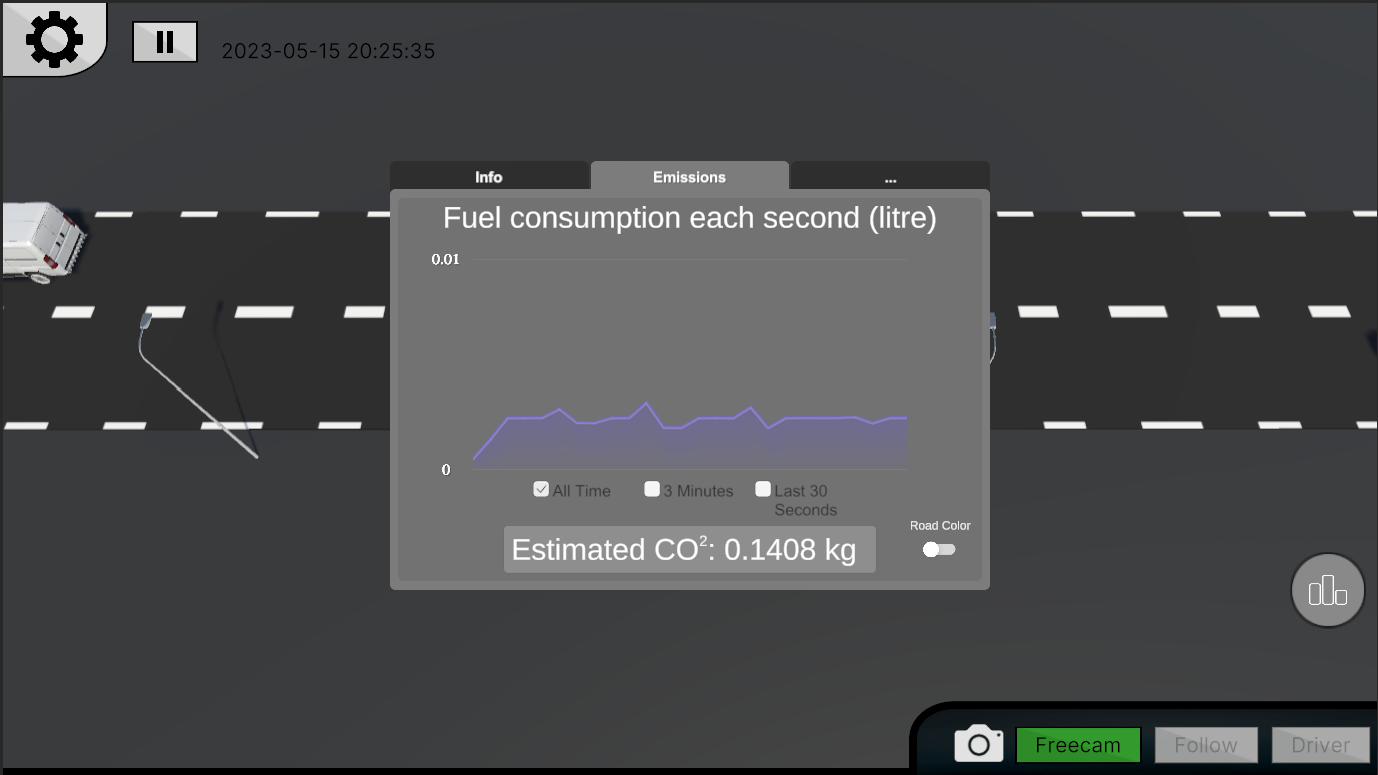
\includegraphics[scale=0.5]{Project_report/figures/method/graph.png}}
        \caption{Graph of fuel consumption}
        \label{fig:Emissions}
    \end{figure}


% WRITTEN BY MARTIN BLOM, 2023
\section{Workflow}
    When developing larger softwares, the amount of work and information can quickly grow beyond the level of ones own comprehension. Therefore, these kinds of projects require rigorous planning and strategising for them to function smoothly.

    To achieve this, a strict workflow framework was developed, where the first step was to analyse the work load and disposable time. This included drafting a time plan for the entire scope of the project, see figure \ref{fig:time-plan}. 

    \begin{figure}[ht]
        \centering
        \fbox{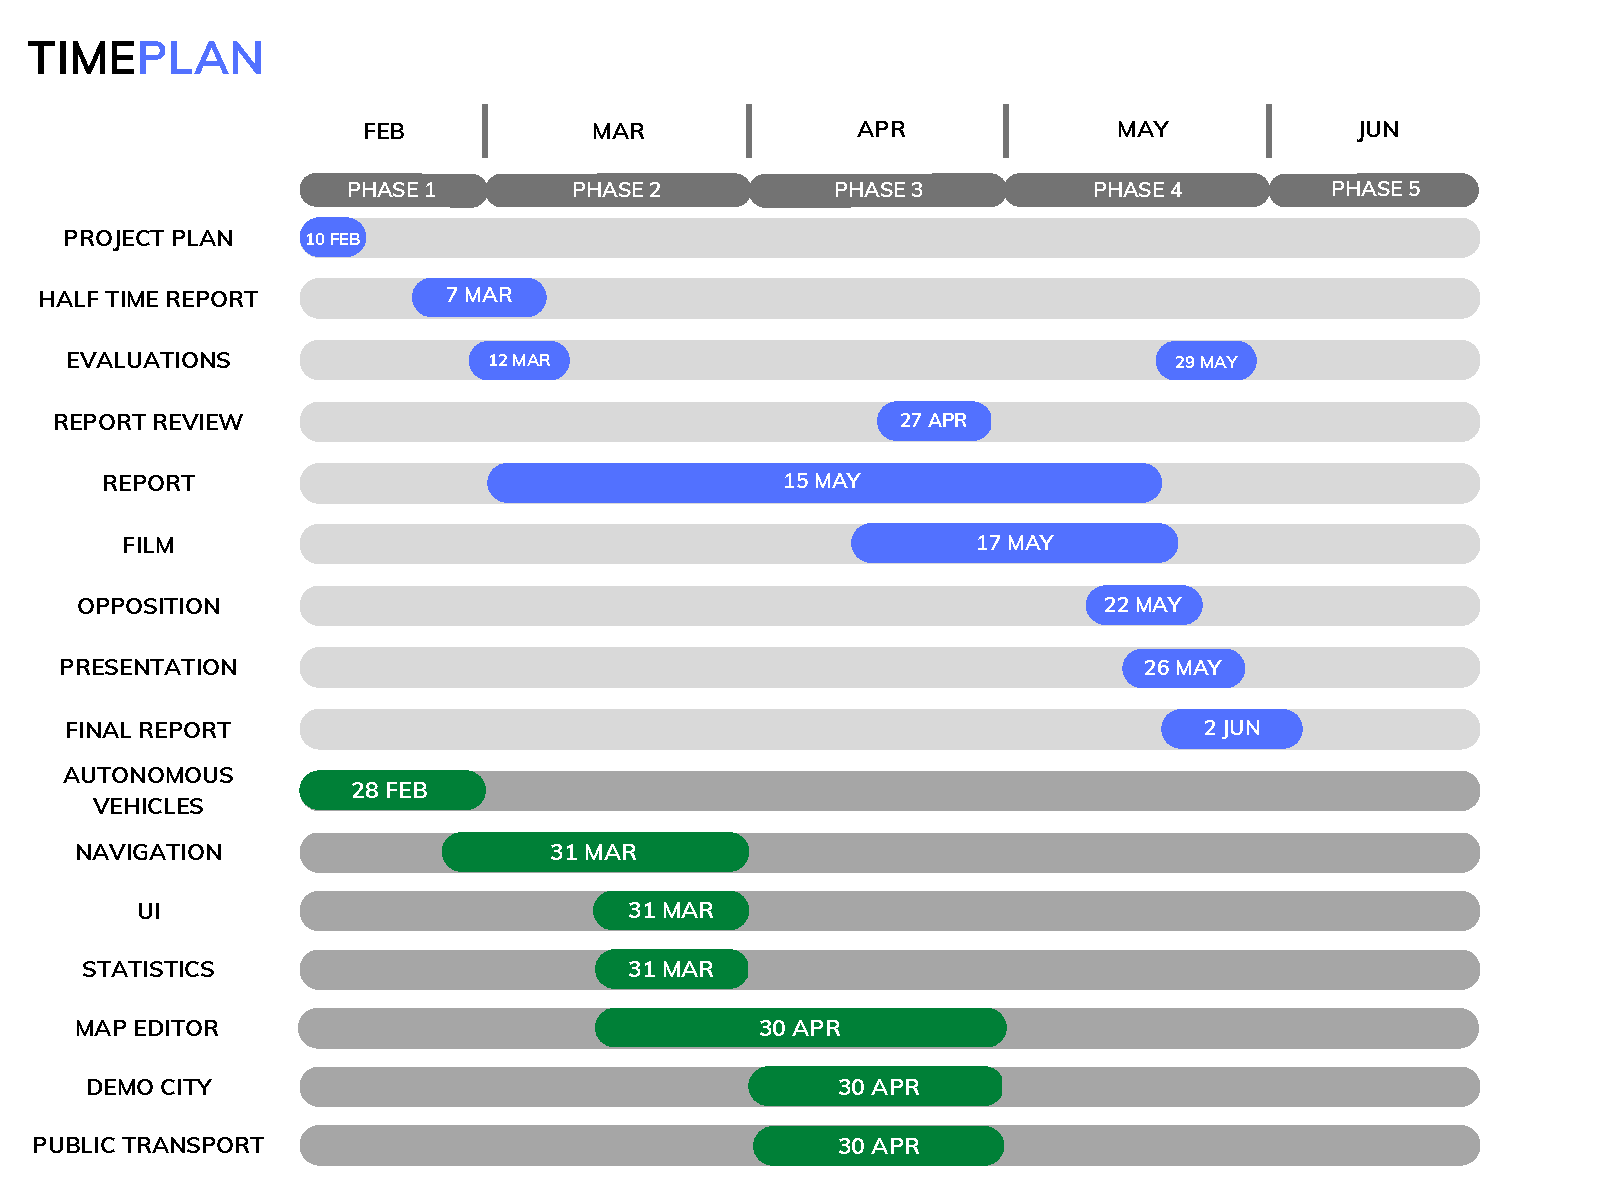
\includegraphics[scale=0.4]{Project_report/appendix/Time_plan.pdf}}
        \caption{Project Time Plan}
        \label{fig:time-plan}
    \end{figure}

    With this system in place, it is easier to keep track of the general progress of the project and plan short term goals. Coincidentally, this is the next step in the workflow model. The short term goals where planned using a scrum framework with weekly sprints, explained later in \ref{sub:weekly-sprints}. These sprints were upheld for the duration of the project to keep a steady flow of progress. Together with the time plan, they create a clear way of visualising the current state of the project.

    The third aspect of the workflow is the approval of progress. As mentioned earlier, a large project requires a substantial amount of planning. The approval of progress can be just as important as the planning and execution itself. Without a proper method of approving new advancements or functionality, the project can quickly falter. If progress never goes through the process of approval, it can lead to problems later on. Evidently, inflexible code can cause issues that are easily preventable through quick inspections. Code can even be considered good, but with no input from the rest of the team, visions of how higher order elements will be implemented can differ. This can implicitly create  more complex problems further on, which can be difficult and time consuming to resolve. To solve this, code reviews were part of the workflow, as explained in section \ref{sub:code-reviewing}.

    % WRITTEN BY MARTIN BLOM, 2023
    \subsection{Weekly Sprints} \label{sub:weekly-sprints}
        The weekly sprint model stems from the scrum framework, which is a framework for developing and sustaining complex products. The sprint model follows 4 repeating stages of development: Planning, Implementation, Review and Retrospect. Each sprint starts out in the planning stage, where a meeting is held to determine the sprint goals. This includes moving or creating stories for the backlog, and the current sprint. The stories are mainly chosen by the project manager, then developed in unison with the scrum master, with continuous input from the rest of the team. The next stage of the sprint is the implementation itself. This is the time where the team focuses solely on delivering completing the tasks for the sprint, and if time allows, work on the backlog.
    
        Next up is the review stage, not to be confused with code reviewing. In this stage another meeting is held, called a "Demo meeting", where all members get to do a small demonstration of their results from the previous sprint. This is an important step to make sure all members understand the new functionality. When a story is regarded as fully complete, it is archived. 
        
        Lastly, during the retrospect stage, the team reflect on the previous sprint and offer any improvements for the next iteration. After the final stage, a new sprint is commenced.

    % WRITTEN BY JAKOB WINDT, 2023 +´Felix 
    \subsection{Trello}
        Early on in the project, it was decided that the workflow should follow scrum and agile software development practices. When doing so, having a scrum-board is essential for implementing the methodologies that accompany these practices. A scrum-board is a visual tool that helps the team keep track of tasks that need to be worked on during the weekly sprints. Each task on the board, which is called a "story", is placed in a column representing the different stages of development depending on where the progress of the task is currently at. Trello is a website that can host scrum-boards in a user-friendly way, which the development team made use of to set up a custom scrum-board template according to their needs\cite{trello}.


    % WRITTEN BY MARCUS SCHAGERBERG, 2023
    \subsection{Code Reviewing} \label{sub:code-reviewing}
        An important part of any larger code base that is being developed and maintained by several developers, is reviewing the code. This serves several purposes, one of which is making sure any new code follows the existing coding standard. However, one of the most useful purposes is that other developers who review the code, could identify potential issues or bugs. This also allows for feedback or solutions to be provided.

        The repository is set up so that the main branch is protected, meaning no new code can be written within the main branch. Instead all code has to be written within separate branches, which are then merged to the main branch. Before any code is merged, it has to be reviewed and approved. This makes sure all code has been viewed by at least two pairs of eyes, increasing the chances of spotting bugs or badly implemented code.

% WRITTEN BY MARCUS SCHAGERBERG, 2023
\section{Testing}
    In order to impartially evaluate the tool and determine if it achieves the purpose, several user testing sessions were held. In these sessions, the users were given a brief explanation of the tool, and then asked to perform a task without any guidance. By analysing the user while trying to perform the tasks, it is possible to follow their intuitions to validate whether the interface is easy to understand and intuitive.

    By asking questions and discussing with the testers during the sessions, we are also able to understand what the users like and dislike, as well as what improvements could be made. By integrating the testing into the development process, we were able to improve the tool and iterate the design before it was finished, thus creating a better result. This created a feedback loop, where we could gather information about what we needed to work on, and improve it according to the feedback before the next testing session. During the next session, we were able to validate whether the changes improved the experience or not. In addition to design related feedback to make the tool intuitive, we also had testing sessions with users experienced with existing transportation planning software in order to assess the features of the tool. This gave insight into what needed to be added, and what could be omitted, as well as what the advantages and disadvantages the tool had compared to existing software.